\documentclass[11pt]{amsart}
\usepackage{amsmath, amssymb, amsthm}
\usepackage{todonotes}
\usepackage{cleveref}

\DeclareMathOperator*{\argmax}{argmax}
\DeclareMathOperator*{\argmin}{argmin}

\theoremstyle{definition}
\newtheorem{definition}{Definition}
\newtheorem{theorem}{Theorem}
\newtheorem{proposition}{Proposition}
\newtheorem{corollary}{Corollary}
\newtheorem{lemma}{Lemma}
\newtheorem{problem}{Problem}
\theoremstyle{remark}
\newtheorem*{remark}{Remark}
\newtheorem*{example}{Example}
\newtheorem*{solution}{Solution}

\title{Prisoner's Dilemma}
\author{Arvid Lunnemark}

\begin{document}
\maketitle

\begin{definition}
  The \textit{prisoner's dilemma} is a symmetric two-player game with two actions, cooperate ($C$) and defect ($D$), where, if player 1 plays $a$ and player 2 plays $b$, player 1 gets payoff 
  \begin{equation*}
    p(a,b) = \begin{cases}
      R &\text{if $a = C, b = C$} \\
      T &\text{if $a = D, b = C$} \\
      S &\text{if $a = C, b = D$} \\
      P &\text{if $a = D, b = D$}
    \end{cases}
  \end{equation*}
  We have $T > R > P > S$, and typically, we have the concrete values $T = 5$, $R = 3$, $P = 1$ and $S = 0$.
\end{definition}

\begin{definition}
  A \textit{strategy} is a Moore machine (finite automaton with outputs) over the input and output alphabet $\{C, D\}$, with probability $1-p$ of following the correct transition and probability $p$ of following the incorrect transition.
\end{definition}

Note: this models an error probability in \textit{perception}. One could also think of an error probability in \textit{outcome}, but it is easy to see that the two are equivalent up to a change of the values of $R, S, T, P$.

\begin{definition}
  Suppose strategy $s_1$ plays against strategy $s_2$. This defines an \textit{$s_1$-$s_2$ graph} which is a Markov chain where each node represents a pair of states $(c_1,c_2)$ where $c_1$ is a state in $s_1$ and $c_2$ is a state in $s_2$. The transition probabilities are defined in the obvious way.
\end{definition}

\begin{definition}
  Let $\pi$ be the stationary distribution achieved by starting in the start state of the \textit{$s_1$-$s_2$ graph}. The \textit{payoff} of strategy $s_1$ when played against strategy $s_2$ is \begin{equation*}
    v_{s_1}(s_2) = \sum \pi_{c_1, c_2} \cdot p(c_1, c_2).
  \end{equation*}
\end{definition}

Note: The graph might be periodic in which case we we will not get a stationary distribution — in that case, however, because of the linearity of the payoffs, we can replace the see that the periodic distribution gets the same time-average value as the stationary distribution that is the mean of the distributions of the periodic end state.

\begin{definition}
  A \textit{population} of strategies $P = (S, f)$ is a set $S$ of strategies and a function $f : S \to (0,1]$ such that $\sum_{s \in S} f(s) = 1$, representing the frequency of each strategy in the population.
\end{definition}

\begin{definition}
  The \textit{fitness} of a strategy $s$ in a population $P = (S, f)$ is \begin{equation*}
    F(s) = \sum_{s' \in S} f(s') v_s(s').
  \end{equation*}
\end{definition}

\begin{definition}
  A strategy $s_1$ is \textit{$\epsilon$-invadable} if there exists a strategy $s_2$ such that in all populations $P$ with $S = \{s_1,s_2\}$ and $f(s_2) \geq \epsilon$, we have \begin{equation}
    \label{fitnesscond}
    F(s_2) > F(s_1)
  \end{equation}
\end{definition}

\begin{definition}
  A strategy $s_1$ is \textit{evolutionarily stable} if there exists parameters $p_0$ and $\alpha$, both in $(0,1)$, such that for all $p < p_0$, and all $\epsilon < \alpha$, $s_1$ is not $\epsilon$-invadable.
\end{definition}

Note: it is easy to see that this is just equivalent to saying that for all $p < p_0$, there exists some $\epsilon$ for which $s_1$ is not $\epsilon$-invadable.

\begin{theorem}
  \label{evolutionarystable1}
  Suppose $s_1$ is evolutionarily stable. Then $\lim_{p \to 0} v_{s_1}(s_1) = R$.
\end{theorem}

\begin{theorem}
  \label{pavlovtheorem}
  The Pavlov strategy, displayed in \cref{pavlovfigure}, is evolutionarily stable.
\end{theorem}

\begin{figure}
  \label{tftfigure}
  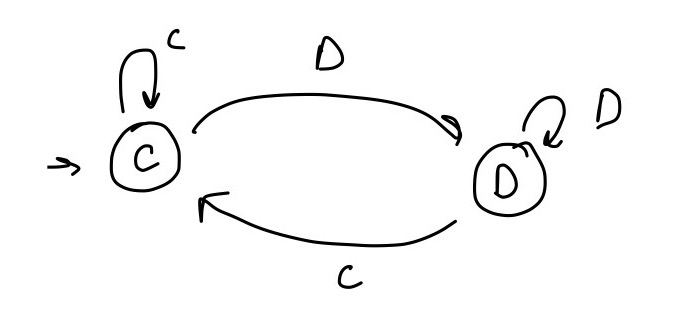
\includegraphics[width=4cm]{tft.jpg}
  \centering
  \caption{TFT.}
\end{figure}
\begin{figure}
  \label{pavlovfigure}
  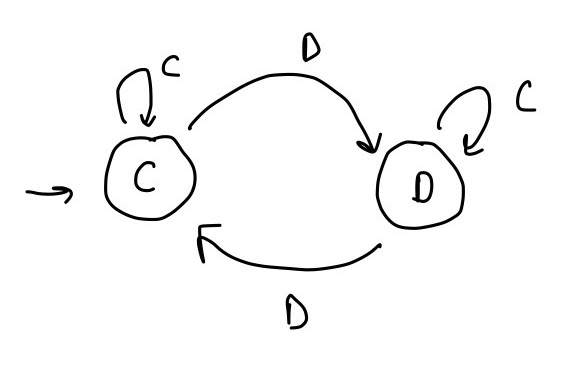
\includegraphics[width=4cm]{pavlov.jpg}
  \centering
  \caption{Pavlov.}
\end{figure}

\begin{remark}
  TFT, displayed in \cref{tftfigure}, is not evolutionarily stable. It has the stationary distribution $(1/4,1/4,1/4,1/4)$ which is smaller than $R$.
\end{remark}

    \begin{proof}[Proof of \cref{evolutionarystable1}]
      Suppose $s_1$ is such that it is not true that \begin{equation*}
        \lim_{p \to 0 } v_{s_1}(s_1) = R
      \end{equation*}
      Note first that $v_{s_1}(s_1)$ is a polynomial in $p$, so the limit exists \todo{Formally prove this!}. Also, by the symmetry of the game, we know that $v_{s_1}(s_1) \leq R$ is always true, so this must mean that $\lim_{p \to 0} v_{s_1}(s_1) < R$ \todo{Formally prove this!}. In particular, then, there exists some $\beta > 0$ such that $v_{s_1}(s_1) = R - \beta$.
      
      We want to prove that $s_1$ is not evolutionarily stable, and to do that, we want to prove that for any sufficiently small $\epsilon$, there exists a strategy $s_2$ that can invade $s_1$.

      We create the strategy $s_2$ as follows. First, copy the entire $s_1$ machine into $s_2$. Suppose the state corresponding to the start state of $s_1$ is $c_s$. Let the output at $c_s$ be $G(c_s)$. Let the node it goes to upon perceiving the opponent move $G(c_s)$ be $T(c_s, G(c_s))$. Then, create a new state $c_0$ that outputs $\lnot G(c_s)$ and has transition $T(c_0, G(c_s)) = T(c_s, G(c_s))$. Create another new state $c_1$. Let $T(c_0, \lnot G(c_s)) = c_1$. Let $T(c_2, \cdot) = c_2$. Let $G(c_2) = C$. This completely describes $s_2$.

      Now, we claim that the payoffs are as follows.
      \begin{equation}
        v_{s_2}(s_1) = (1 - p) \gamma  + p S
      \end{equation}
      \begin{equation}
        v_{s_2}(s_2) = (1-p)^{2} R + 2 (1-p) p (\tfrac{S + T}{2}) + p^2 \gamma
      \end{equation}
      \begin{equation}
        v_{s_1}(s_1) = \gamma
      \end{equation}
      \begin{equation}
        v_{s_1}(s_2) = (1-p) \gamma + p T
      \end{equation}

      Now, we simply compute $F(s_2) - F(s_1)$, and want to show that it is greater than 0 for all $\alpha$ that are sufficiently small.

      \begin{align*}
        F(s_2) - F(s_1) &= \\
        &= (1 - \alpha) \cdot v_{s_2}(s_1) + \alpha \cdot v_{s_2}(s_2) - (1 - \alpha) \cdot v_{s_1}(s_1) - \alpha \cdot v_{s_1}(s_2) \\
        &= 
      \end{align*}

      We can easily see that this works for some small $p$.

    \end{proof}


    \begin{proof}[Proof of \cref{pavlovtheorem}]


    \end{proof}

\end{document}